\newpage
\section{Trigonometry Before Sine and Cosine}	

In this activity, we are going to explore how someone could \textit{understand} that 
\begin{align*}
\sin\left(\frac{\theta}{2}\right) &= \sqrt{\frac{1-\cos(\theta)}{2}}\\
&=\sqrt{\frac{1 - \sqrt{1 - \sin(\theta)^2}}{2}},
\end{align*}
\textit{before} we had the notions of sine and cosine. Consider the following unit circle:
\[
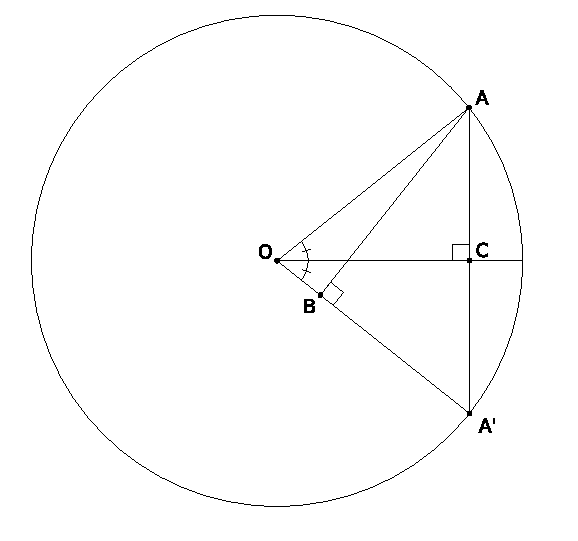
\includegraphics{../graphics/HalfAngleFormula.pdf}
\]


\begin{prob} 
Explain why $\tri OCA$ is similar to $\tri ABA'$.
\end{prob}

\begin{prob} 
Explain why $|BA'| = |CA|\cdot |AA'| = 2|CA|^2$.
\end{prob}

\begin{prob} 
Explain why $|OB|^2 = (1-2|CA|^2)^2$.
\end{prob}

\begin{prob} 
Explain why $|BA|^2 = 1-(1-2|CA|^2)^2$.
\end{prob}


\begin{prob} Solve for $|CA|$ in terms of $|BA|$.
\end{prob}

\begin{prob}
Explain how we have done what we set out to do.
\end{prob}
